
%% ==================================================================================================
%%
\documentclass[12pt]{book}
\usepackage{amsfonts}
\usepackage{amsmath}
\usepackage{amssymb}
\usepackage{graphicx}
\usepackage{hyperref}
\usepackage{float}
\usepackage{verbatim}
\usepackage{multicol} % for side by side \begin{align} equations
\usepackage{xlop} %% for multiplication https://tex.stackexchange.com/questions/11702/how-to-present-a-vertical-multiplication-addition
\usepackage{listings} %% to format generic computer code
\usepackage{lmodern} % for bold teletype font
\usepackage{minted} % colour Java code

\usepackage{tasks}
%\NewTasks[style=enumerate,counter-format=tsk[A].,label-width=3ex]{choice}[\item](4)

%% =======   set page margins    =======
\setlength{\textheight}{10in}
\setlength{\textwidth}{7.4in}
\setlength{\topmargin}{-0.75in}
\setlength{\oddsidemargin}{-0.5in}
\setlength{\evensidemargin}{-0.5in}
\setlength{\parskip}{0.15in}
\setlength{\parindent}{0in}

%%  for European long division
% https://tex.stackexchange.com/questions/432435/how-to-set-up-european-french-style-long-division-in-tex
\newcommand\frdiv[5]{%
    \[
    \renewcommand\arraystretch{1.5}
    \begin{array}{l| l}
    #1 & #2 \\
    \cline{2-2}
    #3 & #4 \\
    \cline{1-1}
    #5 & \\
    \end{array}
    \]
}

%%  for European long division


%% ==================================================================================================

\begin{document}

\newcommand{\reporttitle}{Assignment 2}
\newcommand{\reportauthorOne}{Kien Do}
\newcommand{\cidOne}{300163370}
\input{titlePage/titlepage.txt}



%% ==================================================================================================

%%%%%%%%%%%% PROBLEMS START HERE

\begin{enumerate}
    %% ============================   New Item   ============================
    \item \textbf{Answer}
    
    This is a normal distribution question.\\
    
    Let $E[X] = 12.08$ inches be the mean of a normal variable.\\
    Let $SD[X] = 3.1$ inches be the standard deviation of a normal variable.\\
    Let $VAR[X] = SD[X]^2 = 3.1^2$.\\
    The precipitation of the years 2023 and 2024 are independent.\\
    
    Let $X$ be the yearly precipitation,\\
    $X \sim N(E[X], \text{VAR}[X])$\\
    $X \sim N(12.08,3.1^2) \qquad \xleftarrow[]{\text{by substitution}}$\\
    Let $X_1$ and $X_2$ be 2023 and 2024's precipitation.\\
    
    Since the precipitation for 2023 and 2024 are independent (the probability of precipitation in year 1 doesn't affect year 2, and vice versa), we have that,
    \begin{align*}
        X_1 + X_2 &\sim N(12.08 \times 2, 3.1^2 \times 2)\\
        X_1 + X_2 &\sim N(24.16, 19.22)
    \end{align*}
    
    Therefore, the E[X] for both years is 24.16, and the VAR[X] for both years is 19.22.
    
    We want to find the probability that the total precipitation of both years exceed 25 inches, which is $P((X_1 + X_2) > 25)$. Let $Z = X_1 + X_2$, we have,
    \begin{align*}
        P((X_1 + X_2) > 25) &= P\left(Z > \dfrac{X - E[X]}{SD[X]}\right)\\
        &= P\left(Z > \dfrac{X - E[X]}{\sqrt{\text{VAR[X]}}}\right)\\
        &= P\left(Z > \dfrac{25 - 24.16}{\sqrt{19.22}}\right)\\
        &= P\left(Z > 0.1916\right)\\
        &= 1 - P\left(Z < 0.19\right)\\
        &= 1 - 0.5753 \quad \xleftarrow[\text{ for $Z < 0.19$}]{\text{See Normal Curve table}}\\
        &= 0.4247
    \end{align*}
    $\therefore$ The probability that the total precipitation during the 2 years will exceed 25 inches is 0.4247.
    
    %% ============================   New Item   ============================
    \newpage
    \item \textbf{Answer}
    
    This is a standard error question.
    
    We know the standard deviation and the number of runs to be 1.20 and 40, respectively. So,
    \begin{align*}
        \text{Standard error} &= \dfrac{SD[X]}{\sqrt{n}}\\
        0.18973 &= \dfrac{1.20}{\sqrt{40}} \quad \xleftarrow[]{\text{by substitution}}
    \end{align*}
    Since the runs will be from 1.65 hours to 2.04 hours, we need to find $Z$ for 1.65 and 2.04, $P(1.65 < E[X] < 2.04)$, then find $P(Z_1 < Z < Z_2)$.

    \begin{minipage}{0.45\textwidth}
        \begin{align*}
            Z_1 &= \dfrac{1.65 - 1.82}{0.18973}\\
            Z_1 &= -0.896
        \end{align*}
    \end{minipage}
    \begin{minipage}{0.45\textwidth}
        \begin{align*}
            Z_2 &= \dfrac{2.04 - 1.82}{0.18973}\\
            Z_2 &= 1.1595
        \end{align*}
    \end{minipage}\\
    
    Calculate the probability of the sample mean, $P(Z_1 < Z < Z_2) = P(Z < Z_2) - P(Z < Z_1)$.
    \begin{align*}
        P(-0.896 < Z < 1.1595) &= P(1.1595) - P(-0.896)\\
        P(-0.896 < Z < 1.1595) &= P(1.16) - P(-0.90) \quad \xleftarrow[]{\text{rounding}}\\
        P(-0.90 < Z < 1.16) &= 0.8770 - 0.1841\\
        P(-0.90 < Z < 1.16) &= 0.6929
    \end{align*}
    Therefore, the probability that the sample mean of the next 40 runs will be from 1.65 to 2.04 hours is 0.6929.
    
    %% ============================   New Item   ============================
    \newpage
    \item \textbf{Answer}
    
    We know the sample mean of 20 observations is $\bar{x} = 46$ and the population standard deviation is $\sigma = 9.4$. We also know that the individual measurements follow a normal distribution.\\
    
    We want to know how likely it is that one can obtain $\bar{x} \geq 46$ with $n = 20$ if the population mean is $\mu = 40.38$. If this probability suggests that $\bar{x} = 40.38$ is reasonable, the claim is supported. If the probability is low, one can argue that the data do not support support the claim that $\mu = 40.38$.\\
    
    The probability that we need to compute is $P(|\bar{X} - 40.38|) \geq 40.38$. In other words, if the mean is $\mu = 40.38$, what is the chance that $\bar{X}$ will deviate by as much as $46 - 40.38 = 5.62$?\\
    
    According to CLT, we know that $Z = \dfrac{\bar{X} - \mu}{\sigma / \sqrt{n}}$ has a standard normal distribution, approximately. The desired probability is thus,
    \begin{align*}
        P(|\bar{X}-\mu| \geq 5.62) &= P(\bar{X}-\mu \geq 5.62) + P(\bar{X}-\mu \leq 5.62)\\
        &= P\left( \dfrac{\bar{X} - \mu}{\sigma / \sqrt{n}} \geq \dfrac{5.62}{9.4 / \sqrt{20}}\right) + P\left( \dfrac{\bar{X} - \mu}{\sigma / \sqrt{n}} \leq \dfrac{-5.62}{9.4 / \sqrt{20}}\right)\\
        &= P\left(Z \geq 2.67\right) + P\left(Z \leq -2.67\right)\\
        &= 2P(Z \geq 2.67)\\
        &\approx 2(0.0038) \xleftarrow[\text{ -2.67}]{\text{ z value for}}\\
        &= \dfrac{19}{2500}\\
        &= 0.0076
    \end{align*}
    
    Therefore, the data refutes the treatment plant's claim as one would expect by chance that an $\bar{x}$ would be 40.38 in 19 out of 2500 days.
    
    %% ============================   New Item   ============================
    % \newpage
    % \item \textbf{Answer}
    
    % Placeholder
    
    %% ============================   New Item   ============================
    \newpage
    \item \textbf{Answer}
    
    \begin{enumerate}
        \item Sample mean and sample median.
        
        \begin{minted}[breaklines,frame=single]{R}
> data <- c(136, 182, 143, 147, 173, 151, 158, 160, 161, 171, 163, 155, 165, 167, 173, 174, 152, 181, 144, 181, 185, 156, 169, 188, 190, 205)
> data_mean <- mean(data)
> data_median <- median(data)
> print(data_mean)
[1] 166.5385
> print(data_median)
[1] 166
        \end{minted}
        
        \item Sample variance and sample standard deviation.
        
        \begin{minted}[breaklines,frame=single]{R}
> var(data)
[1] 275.5385
> sd(data)
[1] 16.59935
        \end{minted}
        
        \item Produce a histogram.
        \begin{minted}[breaklines,frame=single]{R}
> hist(data)
        \end{minted}
        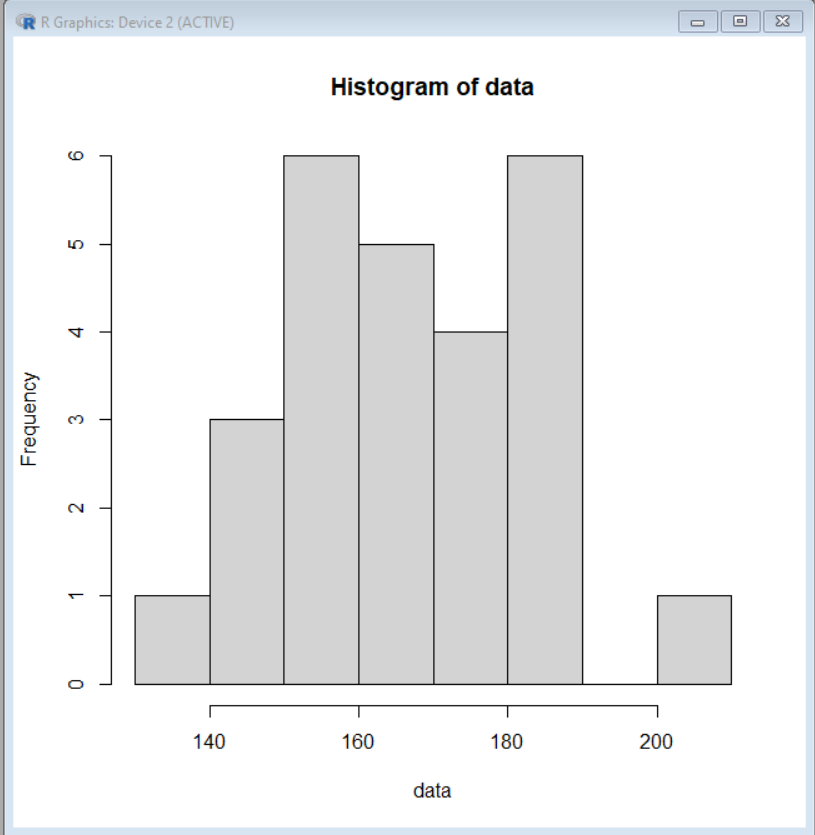
\includegraphics[scale=0.8]{q5_hist.png}
        
        \item Produce a boxplot.
        \begin{minted}[breaklines,frame=single]{R}
> boxplot(data, horizontal = TRUE)
        \end{minted}
        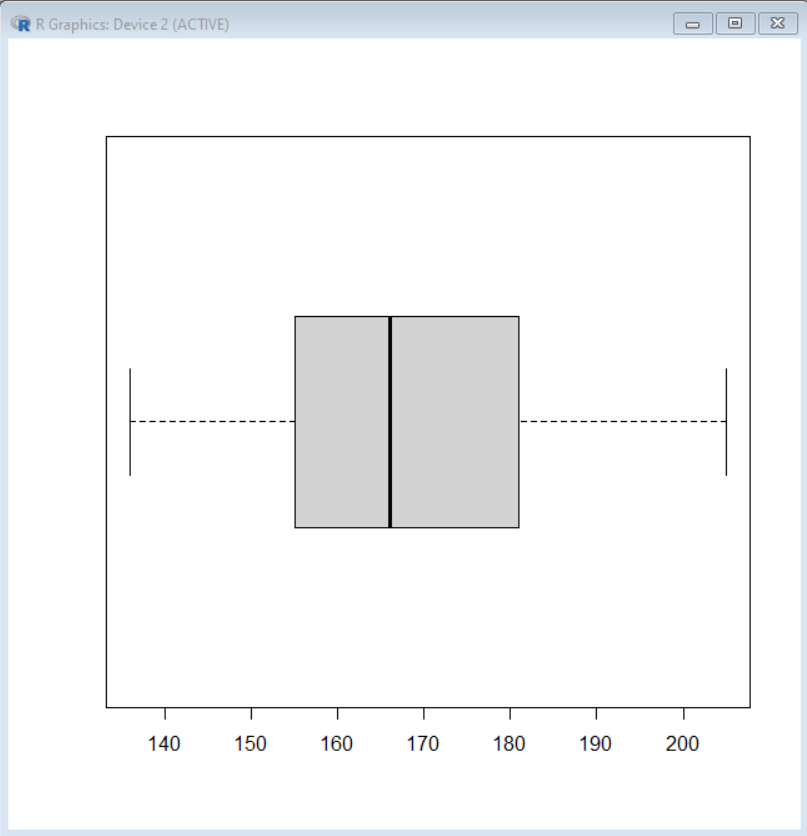
\includegraphics[scale=0.8]{q5_boxplot.png}
        
        \item Find the 95\% and 99\% CIs, assuming that the measurements follow a normal distribution.
        \begin{minted}[breaklines,frame=single]{R}
# Normal population, population standard deviation unknown
> n = 26 # size of sample data set, n
> error <- qt((1+0.95)/(2), n-1) * sd(data)/sqrt(n)
> mean(data) - error
[1] 159.8338
> mean(data) + error
[1] 173.2431 # therefore the 95% CI is (159.8338, 173.2431)
> error <- qt((1+0.99)/(2), n-1) * sd(data)/sqrt(n)
> mean(data) - error
[1] 157.4642
> mean(data) + error
[1] 175.6127 # therefore the 99% CI is (157.4642, 175.6127)
        \end{minted}
        
    \end{enumerate}
    
    %% ============================   New Item   ============================
    \newpage
    \item \textbf{Answer}
    %% https://files.oakland.edu/users/qu/web/STA226winter2010/ch07slide.pdf
    \begin{enumerate}
        \item Calculate minimum sample size needed, given $\sigma = 1.6$, margin of error $d = 0.50$, and confidence level $CL = 99\%$.\\
        
        First, we need to find the z-value for 95\%.
        \begin{align*}
            A &= \dfrac{1+CL}{2}\\
            A &= \dfrac{1+0.95}{2}\\
            A &= 0.975
        \end{align*}
        On the Normal Probability Table, that corresponds to a z-value of $z_{a/2} = 1.96$.
        
        The minimum sample size, $n$, for a $100(1 - \alpha)\%$ confidence interval
        $$\left(\bar{x} - z_{a/2} \times \dfrac{\sigma}{\sqrt{n}} , \bar{x} + z_{a/2} \times \dfrac{\sigma}{\sqrt{n}}\right)$$
        with a margin of error $d$ is $$n = \left( \dfrac{z_{a/2} \, \sigma}{d} \right)^2$$
        Therefore, by substitution, we have,
        \begin{align*}
            n &= \left( \dfrac{z_{a/2} \, \sigma}{d} \right)^2\\
            n &= \left( \dfrac{1.96 \times 1.6}{0.50} \right)^2\\
            n &\approx 40 \quad \xleftarrow[]{\text{ rounded up}}
        \end{align*}
        Therefore, a minimum sample size she needs to take is 40.\\
        
        \item How large is the sample if the confidence level is 99\%?\\
        
        First, we need to find the z-value for 99\%.
        \begin{align*}
            A &= \dfrac{1+CL}{2}\\
            A &= \dfrac{1+0.99}{2}\\
            A &= 0.995
        \end{align*}
        On the Normal Probability Table, that corresponds to a z-value of $z_{a/2} = 2.57$.
    \end{enumerate}
    Therefore, by substitution, we have,
        \begin{align*}
            n &= \left( \dfrac{z_{a/2} \, \sigma}{d} \right)^2\\
            n &= \left( \dfrac{2.57 \times 1.6}{0.50} \right)^2\\
            n &\approx 68 \quad \xleftarrow[]{\text{ rounded up}}
        \end{align*}
        Therefore, a minimum sample size she needs to take is 68.
    
    %% ============================   New Item   ============================
    \newpage
    \item \textbf{Answer}
    
    % We need to use the formula $$\bar{X} \pm z_{a/2} \dfrac{\sigma}{\sqrt{n}}$$
    
    % We can calculate the mean to be
    % $$\bar{X} = \dfrac{5 + 8.5 + 12 + 15 + 7 + 9 + 7.5 + 6.5 + 10.5}{9} = \dfrac{81}{9} = 9$$
    
    % Next, we need to find the 
    
    \begin{enumerate}
        \item Compute a 95\% confidence interval for $\mu$.\\
        
        We need to use the confidence interval formula for $$\mu : \bar{X} \pm t_{a/2}(n-1)\dfrac{S}{\sqrt{n}} \quad \xleftarrow[\text{ is the t-value}]{\text{ the whole } t_{a/2}(n-1)}$$
        
        However, before using that formula, we need to find sample mean $\bar{X}$, sample SD $S$, and $t_{a/2}$.
        
        We can calculate the mean $\bar{E}$ to be
        $$\bar{X} = \dfrac{5 + 8.5 + 12 + 15 + 7 + 9 + 7.5 + 6.5 + 10.5}{9} = \dfrac{81}{9} = 9$$
        
        Find $S^2$ then find $S$.
        \begin{align*}
            S^2 &= \dfrac{1}{n-1} \sum^{n}_{i=1}\left( X_i - \bar{X} \right)^2\\
            S^2 &= \dfrac{1}{9-1} \sum^{n}_{i=1}\left( X_i - 9 \right)^2\\
            S^2 &= 9.5\\
            S &= 3.08
        \end{align*}
        
        Find $t_{a/2}$ by finding $a/2$ and $r$ on the t-distribution Probability Table. Recall $a = 1-CL$ and $r = n-1$.\\
        \begin{minipage}{0.45\textwidth}
            \begin{align*}
                a/2 &= (1-CL)/2\\
                a/2 &= (1-0.95)/2\\
                a/2 &= 0.025
            \end{align*}
        \end{minipage}
        \begin{minipage}{0.45\textwidth}
            \begin{align*}
                r &= n -1\\
                r &= 9 - 1\\
                r &= 8
            \end{align*}
        \end{minipage}\\
        
        Referring to the t-distribution probability table, we have that $t_{a/2} = 2.306$.
        
        Now, calculate a $95\%$ confidence interval for $\mu$ by substituting in relevant values.
        \begin{align*}
            \mu &: \bar{X} \pm t_{a/2}(n-1)\dfrac{S}{\sqrt{n}}\\
            \mu &: (9) \pm (2.306)\dfrac{3.08}{\sqrt{(9)}}\\
            \mu &: 9 \pm 2.367
        \end{align*}
        
        
        \item Compute a $95\%$ confidence interval for $\mu$, if we know $\sigma^2$ = 9.\\
        
        Now that we are given the value of the variance $\sigma^2 = 9$, we can use the following symmetric $100(1-a)\%$ confidence interval formula,
        $$\bar{X} \pm z_{a/2}\dfrac{\sigma}{\sqrt{n}}$$
        We have that $\sigma = \sqrt{\sigma^2} = \sqrt{9} = 3$, and that $z_{a/2} = 1.96$ for a $95\%$ confidence interval. Therefore, by substitution,
        \begin{align*}
            \mu &: \bar{X} \pm z_{a/2}\dfrac{\sigma}{\sqrt{n}}\\
            \mu &: 9 \pm (1.96) \dfrac{3}{\sqrt{3}}\\
            \mu &: 9 \pm 1.96
        \end{align*}
    \end{enumerate}
    
    %% ============================   New Item   ============================
    \newpage
    \item \textbf{Answer}
    
    Find the sample mean of $A$.
    $$\mu_A = \dfrac{36+54+44+52+41+37+53+51}{8} = 46$$
    Find the sample mean of $B$.
    $$\mu_B = \dfrac{52+60+64+44+38+48+68}{7} = 53.43$$
    
    Find the variance for type A, $s^2_A$.
    \begin{align*}
        s^2_A &= \dfrac{1}{n-1} \sum^N_{i=1}(x_i-\bar{x})^2\\
        s^2_A &= \dfrac{(36-46)^2 + ... + (51-46)^2}{8-1} \\
        s^2_A &= 54.85
    \end{align*}
    Find the variance for type B, $s^2_B$.
    \begin{align*}
        s^2_B &= \dfrac{1}{n-1} \sum^N_{i=1}(x_i-\bar{x})^2\\
        s^2_B &= \dfrac{(52-53.43)^2 + ... + (68-53.43)^2}{7-1} \\
        s^2_B &= 120.95
    \end{align*}
    \begin{enumerate}
        
        \item % part a
        
        Since types A and B are normally distributed, and the population variances are equal, $\sigma^2_{A} = \sigma^2_{B}$, the degrees of freedom is then $df=(n_A-1) + (n_B-1)=(8-1)+(7-1)=13$.
        
        The t-value for a $95\%$ confidence level is $t_{0.025} = 2.16$ and the t-value for a $98\%$ confidence level is $t_{0.01} = 2.65$.
        
        We know that the population variances are equal, therefore we can calculate the pooled SD,
        \begin{align*}
            sd_p &= \sqrt{\dfrac{(n_A - 1)s^2_A + (n_B - 1)s^2_B}{df}}\\
            sd_p &= \sqrt{\dfrac{(8 - 1)(54.85) + (7 - 1)(120.95)}{13}}\\
            sd_p &= 9.24
        \end{align*}
        We can now calculate the standard error,
        \begin{align*}
            se &= sd_p\sqrt{\dfrac{1}{n_A}+\dfrac{1}{n_B}}\\
            se &= (9.24)\sqrt{\dfrac{1}{8}+\dfrac{1}{7}}\\
            se &= \dfrac{99}{40}
        \end{align*}
        Calculate the confidence interval for both confidence levels.
        \begin{align*}
            CI &= \left(\bar{X}_A-\bar{X}_B - t_c \times se, \quad \bar{X}_A-\bar{X}_B + t_c \times se\right)\\
            CI_{95\%} &= \left( 46-53.43 - 2.16 \times \dfrac{99}{40}, \quad 46-53.43 + 2.16 \times \dfrac{99}{40} \right)\\
            CI_{95\%} &= (-12.776, \quad -2.084)\\
            CI_{98\%} &= \left( 46-53.43 - 2.65 \times \dfrac{99}{40}, \quad 46-53.43 + 2.65 \times \dfrac{99}{40} \right)\\
            CI_{98\%} &= (-13.99, \quad -0.87)
        \end{align*}
        Therefore, $CI_{95\%} = (-12.776, -2.084)$ and $CI_{98\%} = (-13.99, -0.87)$.
        
        
	   % % "bad" version
    %     \item % part a
        
    %     Since types A and B are normally distributed, and the population variances are equal, $\sigma^2_{A} = \sigma^2_{B}$, the degrees of freedom is then $df=(n_A-1) + (n_B-1)=(8-1)+(7-1)=13$.
        
    %     The t-value for a $95\%$ confidence level is $t_{0.025} = 2.16$ and the t-value for a $98\%$ confidence level is $t_{0.01} = 2.65$.
        
    %     % We know that the population variances are equal, therefore we can calculate the pooled SD,
    %     % \begin{align*}
    %     %     sd_p &= \sqrt{\dfrac{(n_A - 1)s^2_A + (n_B - 1)s^2_B}{df}}\\
    %     %     sd_p &= \sqrt{\dfrac{(8 - 1)(54.85) + (7 - 1)(120.95)}{13}}\\
    %     %     sd_p &= 9.24
    %     % \end{align*}
    %     We know that the population variances are equal, therefore we can now calculate the standard error,
    %     \begin{align*}
    %         se &= sd_p\sqrt{\dfrac{1}{n_A}+\dfrac{1}{n_B}}\\
    %         se &= sd_p\sqrt{\dfrac{1}{8}+\dfrac{1}{7}}\\
    %         se &= sd_p \times \dfrac{15}{56}
    %     \end{align*}
    %     where $sd_p$ is the pooled standard deviation from the population variances.
        
    %     Calculate the confidence interval for both confidence levels.
    %     \begin{align*}
    %         CI &= \left(\bar{X}_A-\bar{X}_B - t_c \times se, \quad \bar{X}_A-\bar{X}_B + t_c \times se\right)\\
    %         CI_{95\%} &= \left( 46-53.43 - 2.16 \times \left( sd_p \times \dfrac{15}{56}\right), \quad 46-53.43 + 2.16 \times \left( sd_p \times \dfrac{15}{56}\right) \right)\\
    %         % CI_{95\%} &= (-12.776, \quad -2.084)\\
    %         CI_{98\%} &= \left( 46-53.43 - 2.65 \times \left( sd_p \times \dfrac{15}{56}\right), \quad 46-53.43 + 2.65 \times \left( sd_p \times \dfrac{15}{56}\right) \right)
    %         % CI_{98\%} &= (-13.99, \quad -0.87)
    %     \end{align*}
    %      $\therefore \, CI_{95\%} = (-7.43 - 0.58se , -7.43 + 0.58se)$ and $CI_{98\%} = (-7.43 - 0.71se, -7.43 + 0.71se)$.
        
        \item % part b
        
        
        The z-value for a $95\%$ confidence level is $\dfrac{1+0.95}{2} = 0.975 \xrightarrow[]{} z_{a/2} = 1.96$ and a z-value for a $97\%$ confidence level is $\dfrac{1+0.97}{2} = 0.985 \xrightarrow[]{} z_{a/2} = 2.17$. Assume $\sigma^2_A = 40$ and $\sigma^2_B = 100$.
        
        The confidence interval for each confidence level,
        \begin{align*}
            CI &= \left( \bar{X}_A-\bar{X}_B - z_{a/2} \sqrt{ \dfrac{\sigma^2_A}{n_A} + \dfrac{\sigma^2_B}{n_B} }, \quad \bar{X}_A-\bar{X}_B + z_{a/2} \sqrt{ \dfrac{\sigma^2_A}{n_A} + \dfrac{\sigma^2_B}{n_B} } \right)\\
            CI_{95\%} &= \left( 46-53.43 - 1.96 \sqrt{ \dfrac{40}{8} + \dfrac{100}{7} }, \quad 46-53.43 + 1.96 \sqrt{ \dfrac{40}{8} + \dfrac{100}{7} } \right)\\
            CI_{95\%} &= (-16.03, 1.18)\\
            CI_{97\%} &= \left( 46-53.43 - 2.17 \sqrt{ \dfrac{40}{8} + \dfrac{100}{7} }, \quad 46-53.43 + 2.17 \sqrt{ \dfrac{40}{8} + \dfrac{100}{7} } \right)\\
            CI_{97\%} &= (-16.96,2.09)
        \end{align*}
        % The confidence interval for a $97\%$ confidence level is then,
        % \begin{align*}
        %     CI &= \left( \bar{X}_A-\bar{X}_B - z_{a/2} \sqrt{ \dfrac{\sigma^2_A}{n_A} + \dfrac{\sigma^2_B}{n_B} }, \quad \bar{X}_A-\bar{X}_B + z_{a/2} \sqrt{ \dfrac{\sigma^2_A}{n_A} + \dfrac{\sigma^2_B}{n_B} } \right)\\
        %     &= \left( 46-53.43 - 2.17 \sqrt{ \dfrac{40}{8} + \dfrac{100}{7} }, \quad 46-53.43 + 2.17 \sqrt{ \dfrac{40}{8} + \dfrac{100}{7} } \right)\\
        %     &= (-16.96,2.09)
        % \end{align*}
        Therefore, the CI for a $95\%$ confidence is $(-16.03, 1.18)$ and the CI for a $97\%$ confidence is $(-16.96,2.09)$.
        
        
    \end{enumerate}
    
    %% ============================   New Item   ============================
    \newpage
    \item \textbf{Answer}
    
    We know that $\bar{E} = 52$ percent with an error of $\pm4$ percent, and that the $CL = 0.95$. Recall the formula,
    $$\hat{P} \pm z_{a/2}\sqrt{\dfrac{\hat{P}(1-\hat{P})}{n}}$$
    Notice that the $\pm z_{a/2}\sqrt{\dfrac{\hat{P}(1-\hat{P})}{n}}$ part is the margin of error and we already know the margin of error is $\pm4$ percent. Therefore, by substitution, we have,
    \begin{align*}
        0.04 &= z_{a/2}\sqrt{\dfrac{\hat{P}(1-\hat{P})}{n}}
    \end{align*}
    Now rearrange the equation and solve for $n$.
    \begin{align*}
        n &= P(1-P) \times \dfrac{z^2}{0.04^2}\\
        n &= (0.52)(1-(0.52)) \times \dfrac{1.96^2}{0.04^2}\\
        n &= 599.28\\
        n &\approx 600 \quad \xleftarrow[\text{ people cannot be a decimal}]{\text{ round to 600 because}}
    \end{align*}
    
    


\end{enumerate}






\end{document} 
